\documentclass[12pt]{gshs_lecture}

\usepackage{datetime}
\usepackage{framed}
\usepackage{verbatim}
\usepackage{color}
\usepackage{ulem}
\usepackage{amsmath,amssymb}
\usepackage{graphicx}
\usepackage{booktabs}
\usepackage{fancyvrb}
\usepackage{hyperref}
\usepackage{subfigure}
\usepackage{pdfpages}
\usepackage{setspace}
\usepackage{listings}

\newdate{date}{04}{06}{2019}

%% Title, Author, Institute, Date %%
\title[]{2019 \LaTeX\ 워크샵}
\subtitle[]{latex.gs.hs.kr}
\author[]{경기과학고 \TeX\ 사용자협회 35기}
\institute[GSHS]{Gyeonggi Science High School\\ for the gifted}
\date[]{\displaydate{date}}

\setbeamertemplate{caption}[numbered]
\renewcommand{\baselinestretch}{1.25}

\newenvironment{codeblock}[1]{
	\begin{block}{#1}
		\setstretch{1.0}
		\begin{small}
}{
		\end{small}
	\end{block}
}

%% Main %%
\begin{document}

%% Title page %%
\begin{frame}[plain]
\titlepage
\end{frame}
\setbeamertemplate{sidebar left}[sidebar theme]

\begin{frame}[t]{Outline}
\tableofcontents%[currentsection]
\end{frame}

\section{What is \LaTeX?}

\begin{frame}[t]{What is \LaTeX ?}
	\begin{itemize}
		\item 1978년 Donald Knuth에 의해 개발된 문서 조판 프로그램인 \TeX 을 사용하기 쉽도록 만든 것
		\item 텍스트를 기반으로 문서 작성(WYSIWYM)
		\item 일정한 형식을 갖춘 문서를 작성하는 데 편함
		\item 특히, 수과학 관련 논문이나 책을 조판하는 데 자주 쓰임
		\item 논문, 책, 발표자료, 시험지, 악보 등 다양한 문서를 작성하는 데 활용 가능
		\item 이 발표자료도 \LaTeX 으로 작성됨!
	\end{itemize}
\end{frame}

\begin{frame}[t]{WYSIWYG vs WYSIWYM}
	문서 편집 프로그램의 두 가지 종류
	\vskip 15pt
	\begin{itemize}
		\item WYSIWYG : What You See Is What You Get
		\begin{itemize}
			\item 한글, MS Word 등
			\item 문서가 만들어지는 과정을 직접 보면서 편집
			\item 키보드 + 마우스 사용
		\end{itemize}
		
		\vskip 15pt
		
		\item WYSIWYM : What You See Is What You Mean
		\begin{itemize}
			\item \LaTeX, HTML, Wiki 등
			\item 문법을 갖춘 코드를 작성하고 컴파일하면 문서로 조판됨
			\item 키보드로만 문서 편집 가능
		\end{itemize}
	\end{itemize}
\end{frame}

\begin{frame}[t]{\LaTeX\ Example}
	\begin{codeblock}{예시 코드}
		\texttt{\textbackslash documentclass\{article\}}
		\vskip 1pc
		\texttt{\textbackslash title\{\textbackslash LaTeX\textbackslash\ Example\}}
		\vskip 1pc
		\texttt{\textbackslash begin\{document\}}
		\vskip 1pc
		\texttt{\textbackslash maketitle}
		\vskip 1pc	
		\texttt{\textbackslash section\{Introduction\}} \\
		\hspace{6mm} \texttt{blah blah blah}
		\vskip 1pc	
		\texttt{\textbackslash section\{Conclusion\}} \\
		\hspace{6mm} \texttt{blah blah blah}
		\vskip 1pc
		\texttt{\textbackslash end\{document\}}
		
	\end{codeblock}
\end{frame}

\begin{frame}[t]{\LaTeX\ Example}
	\begin{framed}
		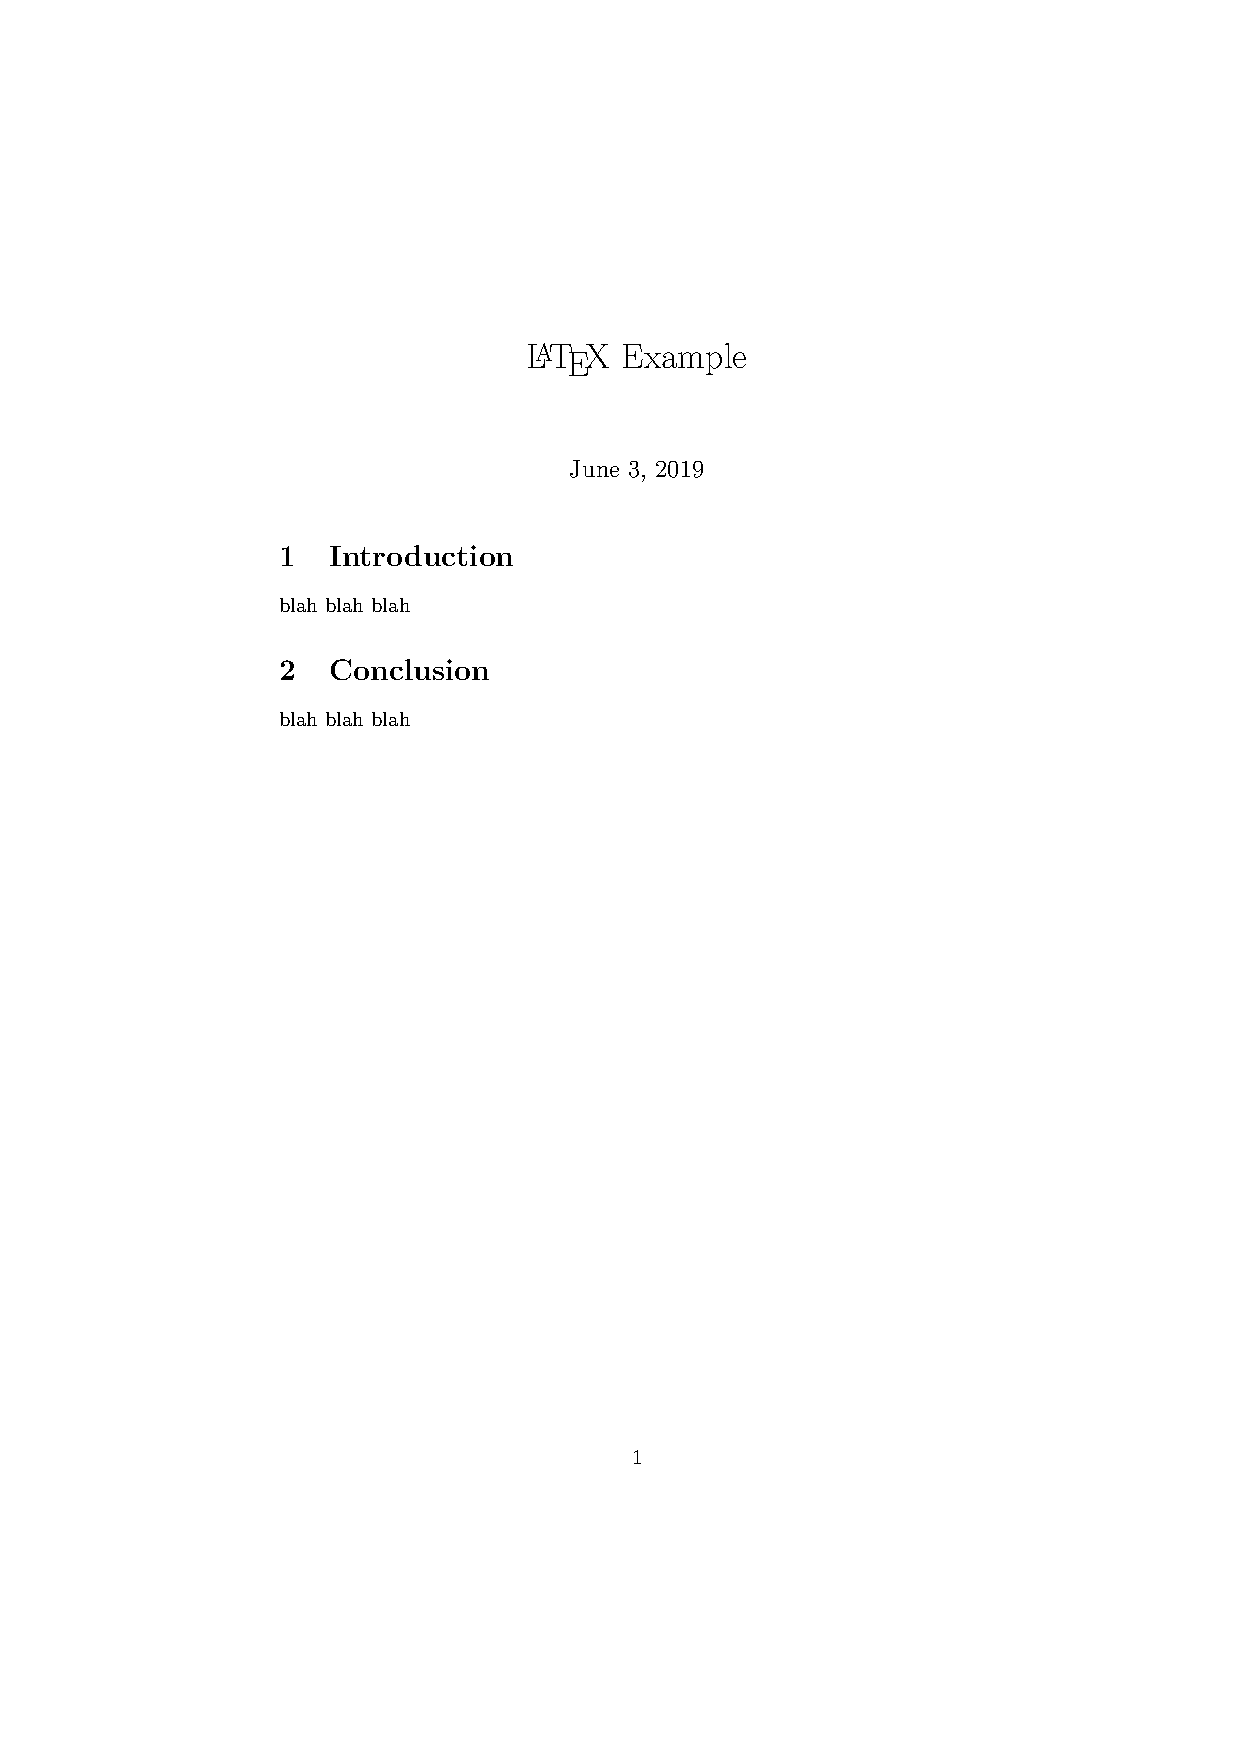
\includegraphics[width=\textwidth,trim={3cm 16.5cm 3cm 4.5cm},clip]{./pdfs/ex1.pdf}
	\end{framed}
\end{frame}

\begin{frame}[t]{Why \LaTeX?}
	\begin{itemize}
		\item \LaTeX의 장점
		\begin{itemize}
			\setstretch{1.5}
			\item 문서가 예쁘고 깔끔하다
			\item 수식 편집이 편하고 빠르다
			\item labeling과 referencing이 편하다
			\item ToC, LoF, LoT 등이 자동화되어 있다
			\item Vector 이미지를 쉽게 삽입할 수 있다
			\item 호환이 잘 된다
			\item 초기 설정을 완료한 후에는 형식에 신경쓸 필요가 없다
			\item 디자인보다 내용에 집중할 수 있다
			\item 다양한 패키지가 존재한다			
		\end{itemize}
	\end{itemize}
\end{frame}

\begin{frame}[t]{Why \LaTeX?}
	\begin{itemize}
		\item \LaTeX의 단점
		\begin{itemize}
			\setstretch{1.5}
			\item 진입장벽이 꽤... 높다
			\item 문법이 비직관적이며, 다양한 명령어들을 알고 있어야 한다
			\item 에러가 발생할 경우 해결하기 어렵다
			\item 구글링이 많이 필요하다			
			\item 문서를 편집하는 도중에 결과를 눈으로 확인할 수 없으며, 수시로 컴파일해야 한다
			\item 그림, 표 등의 위치나 크기를 세밀하게 조절하기 까다롭다
		\end{itemize}
	\end{itemize}
\end{frame}

\section{Examples}

\begin{frame}[t]{Examples}
	\begin{itemize}
		\setstretch{1.5}
		\item GSHS 3D Printer Manual
		\item 졸업논문, 알앤이 보고서
		\item 미적분학II 발표자료
		\item 수학과 산출물
	\end{itemize}
	
\end{frame}

\section{Building a document}

\begin{frame}[t]{새 파일 만들기}
	TexStudio 실행 \textgreater\ File \textgreater\ New
	\vskip 1pc
	
	\LaTeX 으로 문서를 작성하기 위해, 가장 먼저 \texttt{\textbackslash documentclass} 명령어를 사용하여 문서의 클래스를 정의해 주어야 한다.
	
	\vskip 1pc
	
	여기서는 \LaTeX 의 기본 클래스인 \texttt{article}을 사용해보자. \\
	새로 만들어진 파일에 아래 코드를 입력하자.
	
	\vskip 1pc
	
	\begin{codeblock}{}
		\texttt{\textbackslash documentclass\{article\}}
	\end{codeblock}
	
\end{frame}

\begin{frame}[t]{새 파일 만들기}
	본문은 \texttt{\textbackslash begin\{document\}}와 \texttt{\textbackslash end\{document\}} 사이에 작성해야 한다.
	아래와 같이 입력하자.
	
	\vskip 1pc
	
	\begin{codeblock}{}
		\texttt{\textbackslash documentclass\{article\}}
		\vskip 1pc
		{\color{red}
		\texttt{\textbackslash begin\{document\}}
		\vskip 1pc
		\texttt{Hello \textbackslash LaTeX!}
		\vskip 1pc
		\texttt{\textbackslash end\{document\}}
		}
	\end{codeblock}
\end{frame}

\begin{frame}[t]{새 파일 만들기}
	파일을 저장한 뒤, 단축키 F5 (또는 TexStudio 화면 위쪽 도구 바의 초록색 삼각형 두 개가 그려진 버튼)을 눌러 컴파일하자.
	
	\vskip 1pc
	
	화면 오른쪽에 문서의 미리보기가 나타난다. 파일이 저장된 폴더로 가면 pdf 문서가 생성된 것을 확인할 수 있다.
	
	\begin{framed}
		
\includegraphics[width=\textwidth,trim={4cm 23.5cm 4cm 3cm},clip]{./pdfs/ex2.pdf}
	\end{framed}
	
\end{frame}

\begin{frame}[t]{제목 만들기}
	\texttt{\textbackslash title} 명령어로 제목을 설정할 수 있다. \\
	\texttt{\textbackslash author} 명령어로 저자를 설정할 수 있다.
	\vskip 1pc
	\begin{codeblock}{}
		\texttt{\textbackslash documentclass\{article\}}
		\vskip 1pc
		{\color{red}
		\texttt{\textbackslash title\{This is a title.\}} \\
		\texttt{\textbackslash author\{Sebin Kim\}}
		}
		\vskip 1pc
		\texttt{\textbackslash begin\{document\}}
		\vskip 1pc
		\texttt{Hello \textbackslash LaTeX!}
		\vskip 1pc
		\texttt{\textbackslash end\{document\}}
	\end{codeblock}
\end{frame}

\begin{frame}[t]{제목 만들기}
앞에서 설정한 \texttt{title}과 \texttt{author}가 문서에 보이게 하려면 \texttt{\textbackslash maketitle} 명령어가 필요하다.
\vskip 1pc
\begin{codeblock}{}
	\texttt{\textbackslash documentclass\{article\}}
	\vskip 1pc
	\texttt{\textbackslash title\{This is a title.\}} \\
	\texttt{\textbackslash author\{Sebin Kim\}}
	\vskip 1pc
	\texttt{\textbackslash begin\{document\}}
	\vskip 1pc
	{\color{red}
	\texttt{\textbackslash maketitle}
	}
	\vskip 1pc
	\texttt{Hello \textbackslash LaTeX!}
	\vskip 1pc
	\texttt{\textbackslash end\{document\}}
\end{codeblock}
\end{frame}

\begin{frame}[t]{제목 만들기}
	F5를 다시 눌러 결과를 확인하자.
	\vskip 1pc
	\begin{framed}
		
\includegraphics[width=\textwidth,trim={4cm 19cm 4cm 4.5cm},clip]{./pdfs/ex3.pdf}
	\end{framed}
\end{frame}

\begin{frame}[t]{Sections, Subsections}
	\texttt{article} 템플릿에서는 \texttt{\textbackslash section}, \texttt{\textbackslash subsection}, \texttt{\textbackslash subsubsection}, ... 명령어를 통해 절을 나눌 수 있다.
	\vskip 1pc
	\begin{codeblock}{}
		\texttt{...}\\
		\texttt{\textbackslash begin\{document\}}
		\vskip 1pc
		\texttt{\textbackslash maketitle}
		\vskip 1pc
		\texttt{Hello \textbackslash LaTeX!}
		\vskip 1pc
		{\color{red}
		\texttt{\textbackslash section\{The First Section\}}
		\vskip 1pc
		\texttt{\textbackslash section\{The Second Section\}}
		}
		\vskip 1pc
		\texttt{\textbackslash end\{document\}}
	\end{codeblock}
\end{frame}

\begin{frame}[t]{Sections, Subsections}
\begin{codeblock}{}
	\texttt{...}\\
	\texttt{\textbackslash maketitle}
	\vskip 1pc
	\texttt{Hello \textbackslash LaTeX!}
	\vskip 1pc
	\texttt{\textbackslash section\{The First Section\}}
	\vskip 1pc
	{\color{red}
		\texttt{\textbackslash subsection\{Yeah\}} \\
		\texttt{yeah yeah yeah}
		\vskip 1pc
		\texttt{\textbackslash subsection\{Wow\}} \\
		\texttt{wow wow wow}
	}
	\vskip 1pc
	\texttt{\textbackslash section\{The Second Section\}}
	\vskip 1pc
	\texttt{\textbackslash end\{document\}}
\end{codeblock}
\end{frame}

\begin{frame}[t]{Sections, Subsections}
	번호가 자동으로 붙은 것을 확인할 수 있다.
	\vskip 1pc
	\begin{framed}
		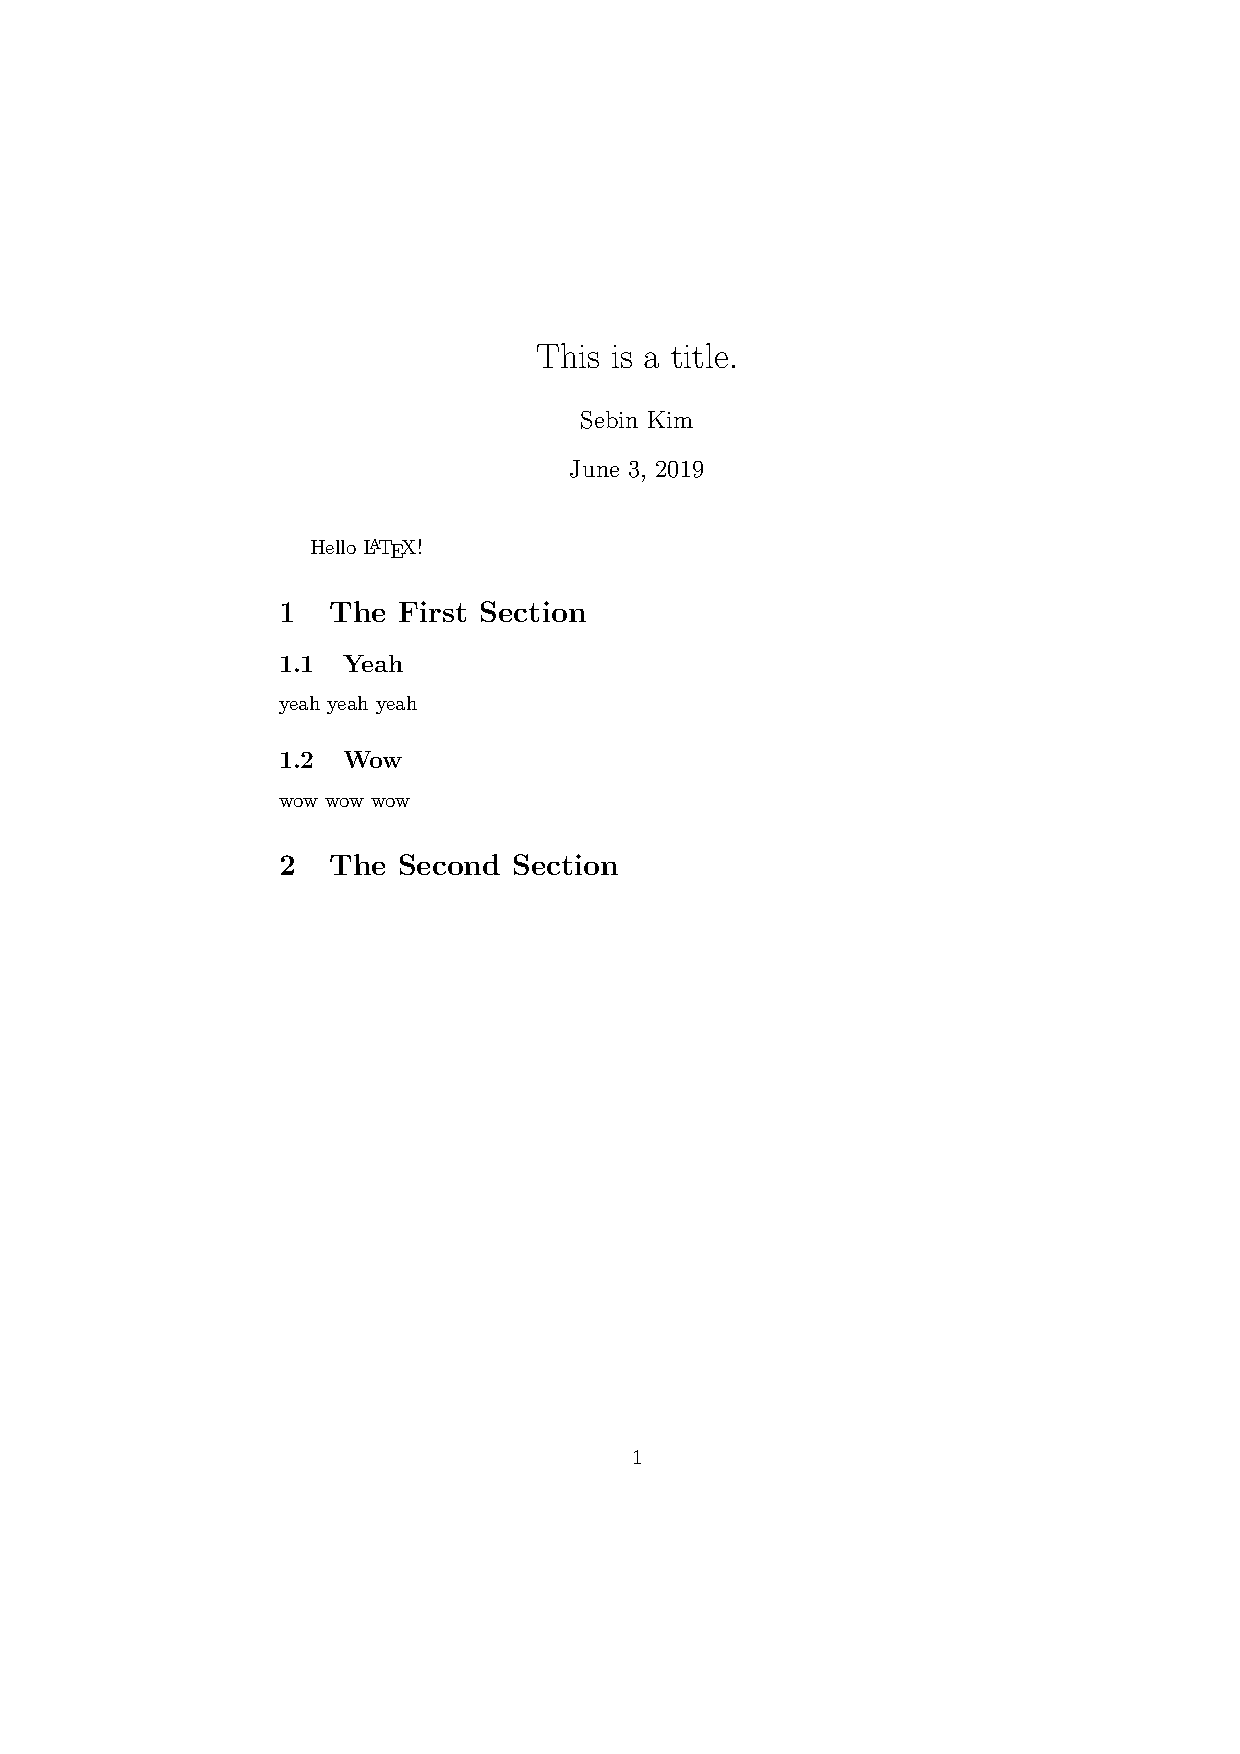
\includegraphics[width=\textwidth,trim={3cm 14.5cm 3cm 7cm},clip]{./pdfs/ex4.pdf}
	\end{framed}
\end{frame}

\begin{frame}[t]{Table of Contents(ToC)}
Table of Contents를 자동으로 생성할 수 있다.
\vskip 1pc
\begin{codeblock}{}
	\texttt{...}\\
	\texttt{\textbackslash begin\{document\}}
	\vskip 1pc
	\texttt{\textbackslash maketitle}
	\vskip 1pc
	\texttt{\textbackslash tableofcontents}
	\vskip 1pc
	\texttt{Hello \textbackslash LaTeX!}
	\vskip 1pc
	{\color{red}
		\texttt{\textbackslash section\{The First Section\}}
		\vskip 1pc
		\texttt{\textbackslash section\{The Second Section\}}
	}
	\vskip 1pc
	\texttt{\textbackslash end\{document\}}
\end{codeblock}
\end{frame}

\begin{frame}[t]{Table of Contents(ToC)}
\begin{framed}
	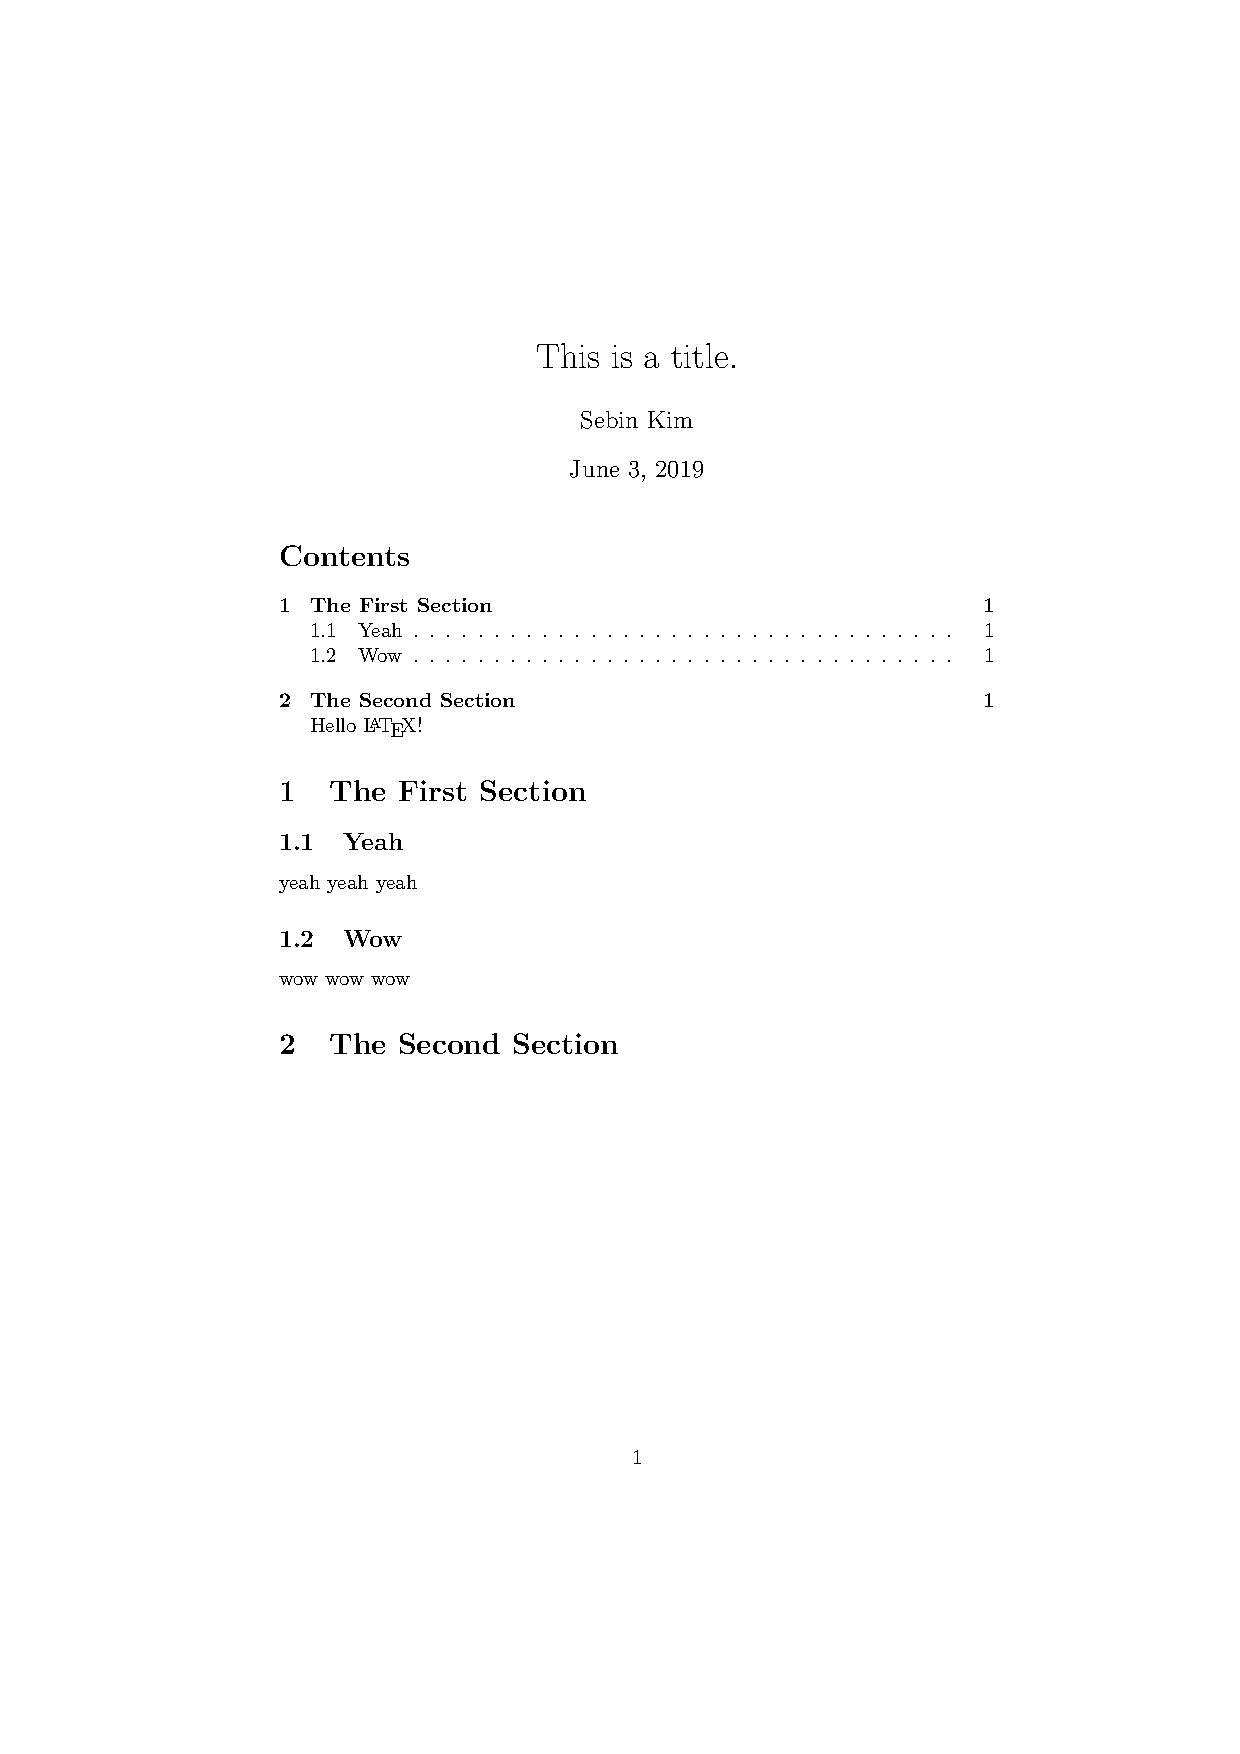
\includegraphics[width=\textwidth,trim={3cm 14.5cm 3cm 6cm},clip]{./pdfs/ex5.pdf}
\end{framed}
\end{frame}

\begin{frame}[t]{환경}
	환경(environment)를 통해 문서 내에 다양한 요소를 추가할 수 있다. 환경은 \texttt{\textbackslash begin\{...\}}으로 시작해 \texttt{\textbackslash end\{...\}}로 끝난다.
	\vskip 1pc
	초록을 작성하기 위해 \texttt{abstract} 환경을 사용해 보자.
	\vskip 1pc
	\begin{codeblock}{}
		\texttt{...}\\
		\texttt{\textbackslash begin\{document\}}
		\vskip 1pc
		\texttt{\textbackslash maketitle}
		\vskip 1pc
		{\color{red}
		\texttt{\textbackslash begin\{abstract\}} \\
		\hspace{6mm} \texttt{green} \\
		\texttt{\textbackslash end\{abstract\}}}
		\vskip 1pc
		\texttt{...}\\
	\end{codeblock}
\end{frame}

\begin{frame}[t]{환경}
\begin{framed}
	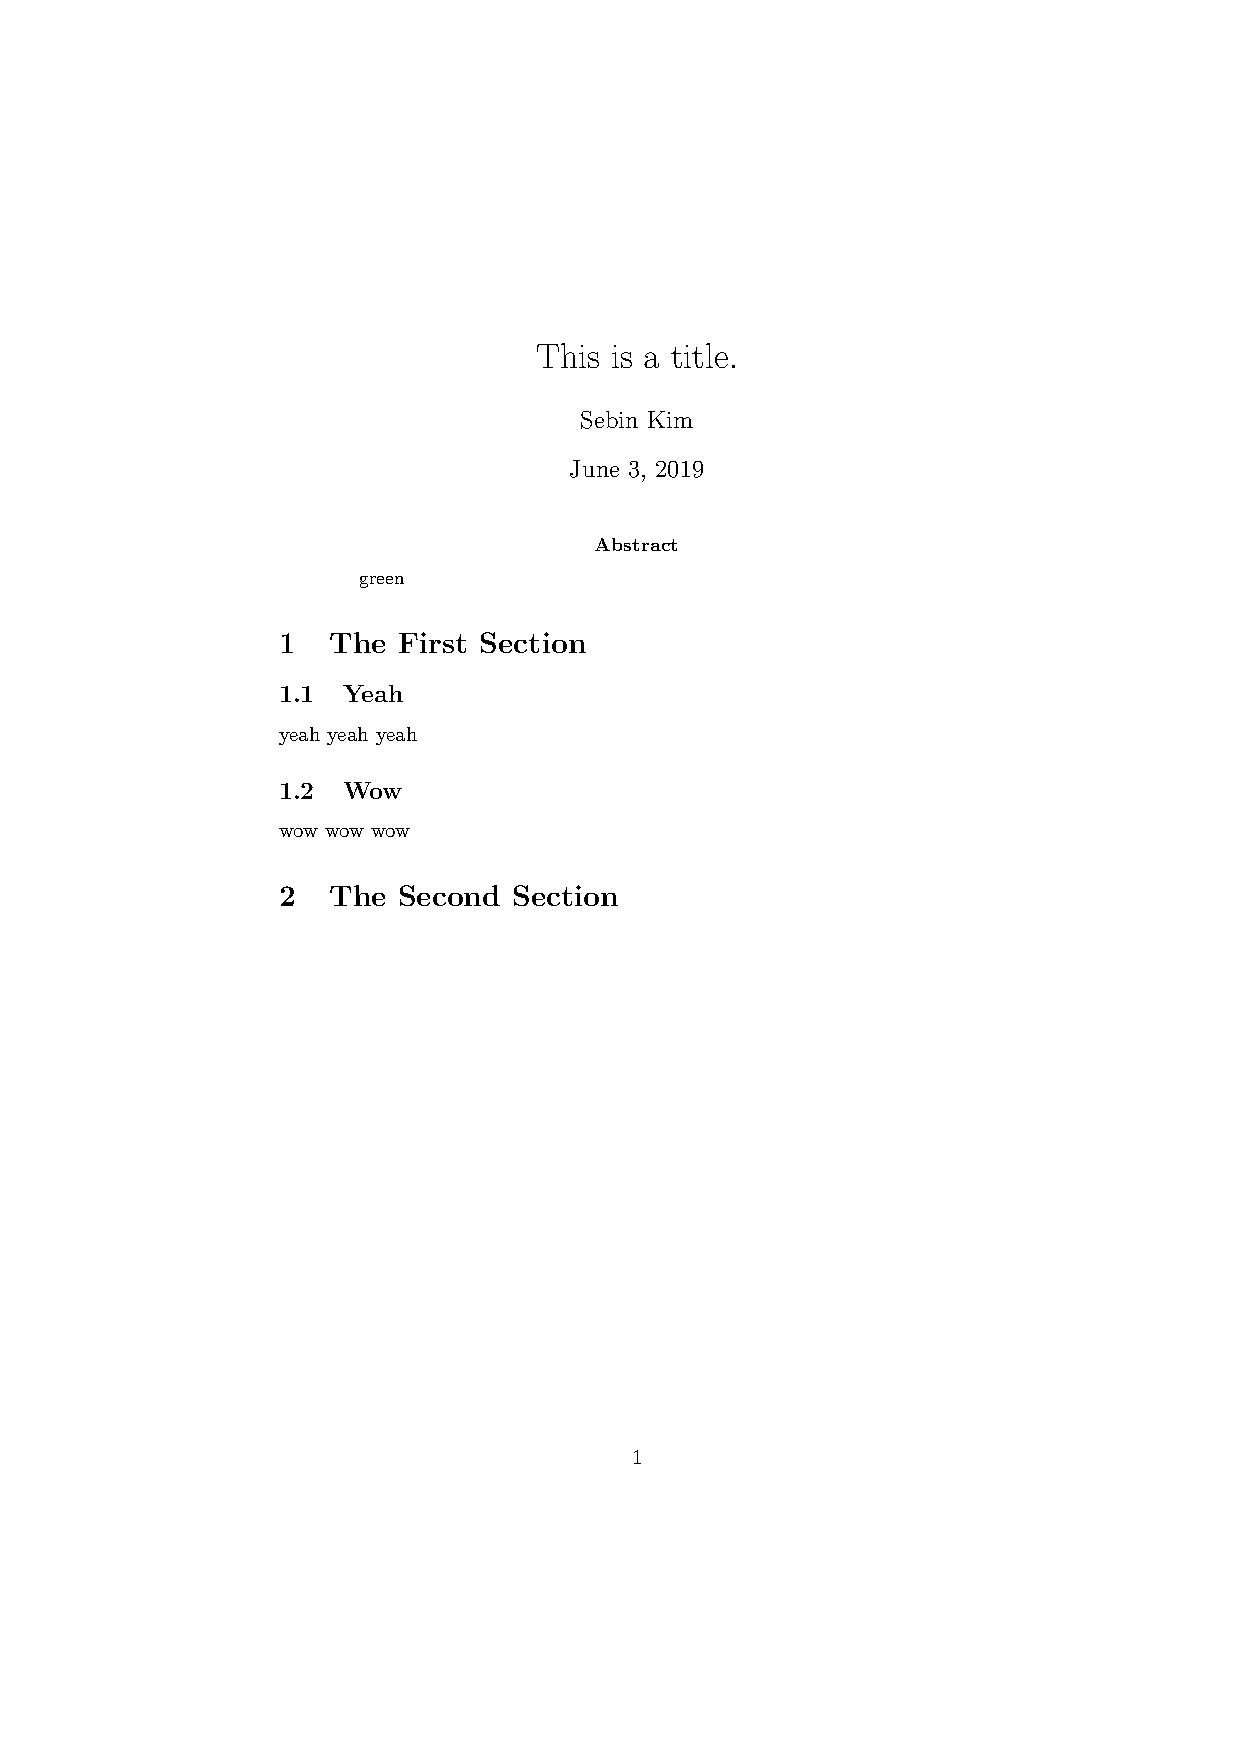
\includegraphics[width=\textwidth,trim={3cm 14.5cm 3cm 6cm},clip]{./pdfs/ex6.pdf}
\end{framed}
\end{frame}

\section{\LaTeX\ Basic}

\begin{frame}[t]{특수문자}
	\TeX 에서 바로 사용할 수 없는 문자 : 
	\begin{center}
		\textbackslash, \#, \$, \%, \&, \{, \}, \_, \textasciitilde, 
		\textasciicircum
	\end{center}
	다음과 같이, 대부분의 경우 단순히 backslash를 붙여주면 된다.
	\begin{center}
		\setstretch{1.0}		
		\texttt{\textbackslash textbackslash}, \texttt{\textbackslash \#}, \texttt{\textbackslash \$}, \texttt{\textbackslash \%}, \texttt{\textbackslash \&},\\
		\texttt{\textbackslash \{}, \texttt{\textbackslash \}}, \texttt{\textbackslash \_},\\
		\texttt{\textbackslash textasciitilde}, \texttt{\textbackslash textasciicircum}
	\end{center}
	
	\LaTeX 에서 특별한 기능을 하는 문자:
	\begin{itemize}
		\item \% : 코드의 주석 처리를 위해 사용된다.
		\item \$ : 수식을 넣기 위해 사용된다.
	\end{itemize}
	Tip : 여러 줄 주석처리는 여기\footnote[frame]{\url{http://bit.ly/2iZ13yn}} 를 참조
\end{frame}

\begin{frame}[t]{띄어쓰기 및 개행}
	\begin{itemize}
		\item \LaTeX\ 코드에서 띄어쓰기를 아무리 많이 해도 결과물에서는 
		띄어쓰기가 한번만 된다.
		\item 여러 번의 띄어쓰기를 위해서는 '\textbackslash'를 쓰면 된다.
		가령 띄어쓰기를 3번 더 하고 싶다면 이 \textbackslash \ \textbackslash \ \textbackslash  \ 렇게 하면\\
		이 \ \ \ 렇게 나온다. \footnote[frame]{\LaTeX 의 기본 띄어쓰기 폭은 한글 글자의 3분의 1이다.}
		\item 여백을 만들어야 할 경우 \textbackslash \texttt{vfill}, \textbackslash \texttt{vspace\{2cm\}} 등을 사용 가능.
	\end{itemize}
\end{frame}

\begin{frame}[t]{띄어쓰기 및 개행}
	\begin{itemize}	
		\item \LaTeX\ 코드 상에서 개행을 한 번만 하면 결과물에 반영되지 않는다.
		\item 개행을 하려면 코드 상에서 줄 끝에 '\textbackslash \textbackslash'를 쓴다.
		\item 빈 줄을 추가하려면 '\textbackslash \texttt{vskip 1pc}'를 사용한다.
		\item 문단을 구분하려면 코드 상에서 개행을 두 번 한다.		
	\end{itemize}
	다양한 개행 방법은 여기\footnote[frame]{\url{http://bit.ly/22ZjIwe}}를 참조 바람.
\end{frame}

\begin{frame}[t]{각주 및 들여쓰기}
	\begin{itemize}
		\item 각주는 단순히 '\textbackslash \texttt{footnote{ ...}}' 와 같이 사용하면 된다. 단, 표에서 사용할 경우 문제가 발생할 수 있다.
		\vskip 1pc
		
		\item 들여쓰기는 기본적으로 조정이 되지만, 처음에 익숙하지 않을 때는 단순히 
		\textbackslash \texttt{indent}, \textbackslash \texttt{noindent}로 강제 조정할 수 있다.
		
		\vskip 1pc
		\item 2회 개행은 문단 나눔이기 때문에 들여쓰기가 되지만, '\textbackslash \textbackslash'로 
		개행하면 들여쓰기가 없다. 
	\end{itemize}
	
\end{frame}

\begin{frame}[t]{문서의 정렬}
	\begin{flushleft}
		좌측 정렬
	\end{flushleft}
	\begin{flushright}
		우측 정렬
	\end{flushright}
	\begin{center}
		중앙 정렬
	\end{center}
	각각 flushleft, flushright, center 환경을 사용하면 된다.
	
	\begin{codeblock}{중앙 정렬}
	\textbackslash \texttt{begin\{center\}}\\
	\hspace{6mm} 중앙 정렬된 텍스트...\\
	\textbackslash \texttt{end\{center\}}
	\end{codeblock}
\end{frame}

\begin{frame}[t]{글꼴 및 색상}
	\begin{itemize}
		\item \textbf{굵게} : \textbackslash \texttt{textbf\{ ... \}}
		\item \textit{이탤릭} : \textbackslash \texttt{textit\{ ... \}}
		\item \textsf{산세리프}\footnote[frame]{본 문서는 beamer class 를 
			사용하기 때문에 기본 폰트가 산세리프이다. 한글의 경우 
			나눔고딕.} : \textbackslash \texttt{textsf\{ ... \}}
		\item {\color{blue} 색상} : color 패키지를 사용,
		\textbackslash \texttt{color\{blue\} ... }
	\end{itemize}
	kotexlive 2013 기준으로, \TeX 의 기본 한글글꼴은 네이버에서 배포한 나눔명조 및 나눔고딕이다. 영어 기본 글꼴은 `Computer Modern' 이고, 필요할 경우 해당 package 를 사용하여 Times New Roman 을 사용할 수 있다. 사용방법 : \footnote[frame]{\url{http://pastebin.com/fZphiXGT}}
\end{frame}

\begin{frame}[t]{열거 환경 : itemize / enumerate}
	\begin{itemize}
		\item 한국의 수도는 서울이다.
		\item 미국의 수도는 워싱턴이다.
		\item 프랑스의 수도는 파리이다.
	\end{itemize}
	\begin{enumerate}
		\item 컴퓨터를 켠다.
		\item \LaTeX 을 실행한다.
		\item 졸업논문을 작성한다.
	\end{enumerate}

	\begin{codeblock}{열거}
		\textbackslash \texttt{begin\{itemize\}}\\
		\hspace{6mm} \textbackslash \texttt{item} 첫 번째 아이템...\\
		\hspace{6mm} \textbackslash \texttt{item} 두 번째 아이템...\\
		\textbackslash \texttt{end\{itemize\}}
	\end{codeblock}
\end{frame}

\section{Equations}

\begin{frame}[t]{Equations --- (1)}
	
	\begin{itemize}
		\item amsmath 패키지를 불러오자
	\end{itemize}
	\textbackslash\texttt{usepackage\{amsmath\}}
	\vskip 1pc
	
	\begin{enumerate}
		\item \texttt{\$ ... \$} : 행 내 수식
		\item \texttt{\textbackslash( ... \textbackslash)} : 행 내 수식
		\item \texttt{\textbackslash[ ... \textbackslash]} : 표시형 수식, 번호 없음
		\item equation, align, gather : 추후에 설명
	\end{enumerate}
	
	\begin{itemize}
		\item 수식 문법은 TeXstudio의 가장 왼쪽 바에서 확인 가능
	\end{itemize}
	
\end{frame}

\begin{frame}[t]{Examples}
	
	\[1 + 2 = 3\]
	\[f(x) = \frac{1}{x}\]
	\[e^{i\pi} + 1 = 0\]
	\[\sqrt[3]{8} = 2\]
	
	\begin{codeblock}{수식 입력}
		\texttt{\textbackslash[1 + 2 = 3\textbackslash]}\\
		\texttt{\textbackslash[f(x) = \textbackslash frac\{1\}\{x\}\textbackslash]}\\
		\texttt{\textbackslash[e\^{}\{i\textbackslash pi\} + 1 = 0\textbackslash]}\\
		\texttt{\textbackslash[\textbackslash sqrt[3]\{8\} = 2\textbackslash]}
	\end{codeblock}
\end{frame}

\begin{frame}[t]{Examples}
	
	\[\sum_{k=1}^{n}{k} = \frac{n(n+1)}{2}\]
	\[\int_{-\infty}^{\infty}{e^{-x^2} dx} = \sqrt{\pi}\]
	
	\begin{codeblock}{수식 입력}
		\texttt{\textbackslash[\textbackslash sum\_\{k = 1\}\^{}\{n\}\{k\} = \textbackslash frac\{n(n + 1)\}\{2\}\textbackslash]}
		\texttt{\textbackslash[\textbackslash int\_\{-\textbackslash infty\}\^{}\{\textbackslash infty\}\{e\^{}\{-x\^{}2\} dx\}\\= \textbackslash sqrt\{\textbackslash pi\}\textbackslash]}
	\end{codeblock}
	
\end{frame}

\begin{frame}[t]{Equations --- (2)}
	
	\begin{itemize}
		\item equation : 표시형 수식, 번호 있음
		\item align : 수식을 여러 줄에 걸쳐 예쁘게 정리해 줌
		\item gather : 여러 줄로 이루어진 수식을 가운데 정렬
		\vskip 1.5pc
		\item \textbackslash ref\{\}, \textbackslash eqref\{\}을 이용해 번호 참조 가능
		\item 위 환경에서 *을 붙이면 번호가 사라짐
	\end{itemize}
	
\end{frame}

\begin{frame}[t]{Examples}
	
	\begin{equation}
	e^{i\theta} = \cos{\theta} + i\sin{\theta}
	\label{eq1}
	\end{equation}
	
	\begin{center}
		오일러의 공식은 \eqref{eq1}과 같다.
	\end{center}
	
	\begin{codeblock}{equation + label}
		\texttt{\textbackslash begin\{equation\}}\\
		\hspace{6mm} \texttt{e\^{}\{i\textbackslash theta\} = \textbackslash cos\{\textbackslash theta\} + i\textbackslash sin\{\textbackslash theta\}}\\
		\hspace{6mm} \textbackslash \texttt{label\{eq1\}} \\
		\texttt{\textbackslash end\{equation\}} \\		
		\texttt{오일러의 공식은 \textbackslash eqref\{eq1\}과 같다.}
	\end{codeblock}
	
\end{frame}

\begin{frame}[t]{Examples}
	
	\begin{align*}
	(x + 1)^2 &= (x + 1)(x + 1)\\
	&= x^2 + x + x + 1\\
	&= x^2 + 2x + 1
	\end{align*}
	
	\begin{codeblock}{align}	
		\texttt{\textbackslash begin\{align*\}}\\
		\hspace{6mm} \texttt{(x + 1)\^{}2 \&= (x + 1)(x + 1) \textbackslash\textbackslash}\\
		\hspace{6mm} \&=\texttt{x\^{}2 + x + x + 1 \textbackslash\textbackslash}\\
		\hspace{6mm} \&=\texttt{x\^{}2 + 2x + 1}\\
		\texttt{\textbackslash end\{align*\}}
	\end{codeblock}
	
\end{frame}

\begin{frame}[t]{Examples}
	
	\begin{gather*}
	2x + y = 4\\
	x + 4y + z = 10
	\end{gather*}
	
	\begin{codeblock}{gather}	
		\texttt{\textbackslash begin\{gather*\}}\\
		\hspace{6mm} \texttt{2x + y = 4 \textbackslash\textbackslash}\\
		\hspace{6mm} \texttt{x + 4y + z = 10 \textbackslash\textbackslash}\\
		\texttt{\textbackslash end\{gather*\}}
	\end{codeblock}
	
\end{frame}


\section{Figures, Tables}

\begin{frame}[t]{그림 삽입하기}
	그림을 삽입하기 위해서는 \texttt{graphicx} 패키지가 필요하다.
	
	문서 맨 위, \texttt{\textbackslash documentclass} 아래에 다음 코드를 추가해주자.
	
	\vskip 1pc
	
	\begin{codeblock}{}
		\texttt{\textbackslash usepackage\{graphicx\}}
	\end{codeblock}
\end{frame}

\begin{frame}[t]{그림 삽입하기}
	
	\begin{figure}[htbp]
		\centering
		
\includegraphics[width=.2\textwidth]{./pictures/GSW_logo.jpg}
		\caption{GSW Logo}
		\label{GSW}
	\end{figure}
	
	\begin{codeblock}{그림 삽입}
		\textbackslash \texttt{begin\{figure\}[htbp]}\\
		\hspace{6mm} \textbackslash \texttt{centering}\\
		\hspace{6mm} \textbackslash \texttt{includegraphics[width=.2\textbackslash textwidth]\{GSW.jpg\}}\\
		\hspace{6mm} \textbackslash \texttt{caption\{GSW Logo\}}\\
		\hspace{6mm} \textbackslash \texttt{label\{GSW\}}\\
		\textbackslash \texttt{end\{figure\}}
	\end{codeblock}
\end{frame}

\begin{frame}[t]{h,t,b,p 옵션}
	'\textbackslash \texttt{begin\{figure\}}' 바로 뒤의 대괄호에 등장하는 옵션에 대해 알아보자.
	\begin{table}
		\centering
		\begin{tabular}{|c|p{0.8\textwidth}|}
			\hline
			h & 개체를 코드의 위치(여기 : \textbf{h}ere)에 놓음 \\
			\hline
			t & 개체를 페이지의 맨 위쪽(\textbf{t}op)에 놓음 \\
			\hline
			b & 개체를 페이지의 맨 아래쪽(\textbf{b}ottom)에 놓음 \\
			\hline
			p & 개체를 특정 페이지(\textbf{p}age)에 놓음. 별다른 설정이 없으면 문서의 맨 뒤. \\
			\hline
			! & \LaTeX 에서 미리 설정해놓은 일부 서식을 무시하고(ex. 텍스트 여백) 놓음\\
			\hline
		\end{tabular}
	\end{table}
\end{frame}

\begin{frame}[t]{Subfigure}
	
	\begin{figure}[h]
		\centering
		\subfigure[h][GSW]{
\includegraphics[width=.2\textwidth]{./pictures/GSW_logo.jpg}}
		\centering
		\subfigure[h][TOR]{
\includegraphics[width=.2\textwidth]{./pictures/Tor_logo.png}}
		\caption{NBA FINAL}
		\label{NBAFINAL}
	\end{figure}
	
\end{frame}

\begin{frame}[t]{Subfigure}
	
	\begin{itemize}
		\item subfigure package를 import 해야 한다.
	\end{itemize}

	\hspace{6mm} $\rightarrow$ \textbackslash \texttt{usepackage\{subfigure\}}
	
	\begin{codeblock}{subfigure}
		\textbackslash \texttt{begin\{figure\}[htbp]}\\
		\hspace{6mm} \textbackslash \texttt{centering}\\
		\hspace{6mm} \textbackslash \texttt{subfigure[h][GSW]\{\textbackslash includegraphics\\
			\hspace{6mm} [width=.2\textbackslash textwidth]\{GSW.jpg\}\}}\\
		\hspace{6mm} \textbackslash \texttt{centering}\\
		\hspace{6mm} \textbackslash \texttt{subfigure[h][TOR]\{\textbackslash includegraphics\\
			\hspace{6mm} [width=.2\textbackslash textwidth]\{TOR.jpg\}\}}\\
		\hspace{6mm} \textbackslash \texttt{caption\{NBA FINAL\}}\\
		\hspace{6mm} \textbackslash \texttt{label\{NBAFINAL\}}\\
		\textbackslash \texttt{end\{figure\}}	
	\end{codeblock}
	
\end{frame}

\begin{frame}[t]{표 삽입}
	
	\begin{itemize}
		\item \LaTeX 에서 코드로 작성
		\item \LaTeX\ Table Generator\footnote[frame]{\url{https://www.tablesgenerator.com/}}을 이용
	\end{itemize}
	
	\begin{table}[h]
		\centering
		\begin{tabular}{|l|c|r|}
			\hline
			나라&수도&대륙\\
			\hline
			\hline
			대한민국&서울&아시아\\
			\hline
			미국&워싱턴&아메리카\\
			\hline
		\end{tabular}
		\caption{나라 정보}
		\label{countries}
	\end{table}
\end{frame}

\begin{frame}[t]{표 삽입}
	
	\begin{codeblock}{표 삽입}
		\textbackslash \texttt{begin\{table\}[h]}\\
		\hspace{6mm} \textbackslash \texttt{centering}\\
		\hspace{6mm} \textbackslash \texttt{begin\{tabular\}\{|l|c|r|\}}\\
		\hspace{14mm} \textbackslash \texttt{hline}\\
		\hspace{14mm} \texttt{나라\&수도\&대륙\textbackslash \textbackslash}\\
		\hspace{14mm} \textbackslash \texttt{hline}\\
		\hspace{14mm} \textbackslash \texttt{hline}\\
		\hspace{14mm} \texttt{대한민국\&서울\&아시아\textbackslash \textbackslash}\\
		\hspace{14mm} \textbackslash \texttt{hline}\\
		\hspace{14mm} \texttt{미국\&워싱턴\&아메리카\textbackslash \textbackslash}\\
		\hspace{14mm} \textbackslash \texttt{hline}\\
		\hspace{6mm} \textbackslash \texttt{end\{tabular\}}\\
		\hspace{6mm} \textbackslash \texttt{caption\{나라 정보\}}\\
		\hspace{6mm} \textbackslash \texttt{label\{countries\}}\\
		\textbackslash\texttt{end\{table\}}
	\end{codeblock}
	
\end{frame}


\section{Referencing}

\begin{frame}[t]{라벨링}
	
	\begin{itemize}
		\item 위에서 그림, 표를 삽입할 때 \textbackslash \texttt{label\{...\}}을 썼던 이유는?
		\item 자동 라벨링을 위함이다.
		\item \LaTeX 에서는 라벨링을 하면 자동으로 순서를 매겨주고 tag를 사용해 본문에 표시한다.
		\item \textbackslash \texttt{label\{...\}} $\leftrightarrow$ \textbackslash \texttt{ref\{...\}}
		\item 그림, 표 등에서는 \textbackslash \texttt{ref\{...\}} 사용
		\item 수식에서는 \textbackslash \texttt{eqref\{...\}} 사용
		\item \textbackslash \texttt{ref\{GSW\}} $\rightarrow$ '\ref{GSW}'
		\item \textbackslash \texttt{ref\{NBAFINAL\}} $\rightarrow$ '\ref{NBAFINAL}'
		\item \textbackslash \texttt{ref\{countries\}} $\rightarrow$ '\ref{countries}'
	\end{itemize}
	
\end{frame}

\begin{frame}[t]{라벨링}
	\begin{figure}[htbp]
		\centering
		
\includegraphics[width=.2\textwidth]{./pictures/GSW_logo.jpg}
		\caption{GSW Logo}
		\label{GSW2}
	\end{figure}

	그림 \ref{GSW2}은 GSW의 로고이다.
	
	\vskip 1pc	
	
	\begin{codeblock}{라벨링}
		\texttt{그림 \textbackslash ref\{GSW\}은 GSW의 로고이다.}
	\end{codeblock}
	
\end{frame}

\begin{frame}[t]{참고문헌}
	
	참고문헌 역시 \LaTeX 은 자동으로 정리해준다!\\
%	\hspace{6mm} $\rightarrow$ bibTeX
	\vskip 2pc
	\begin{figure}[h]
		\centering
			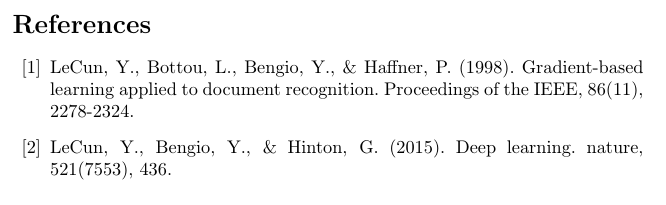
\includegraphics[width=.8\textwidth]{./pictures/Ref.png}
		\caption{References}
		\label{Ref}
	\end{figure}
	
%	\includepdf[pages={1}]{./bibtex/bib.pdf}
	
\end{frame}

\begin{frame}[t]{참고문헌}
	\begin{codeblock}{참고문헌}
		\textbackslash \texttt{begin\{thebibliography\}\{99\}}\\
		\hspace{6mm} \textbackslash \texttt{bibitem\{CNN\} LeCun, Y., Bottou, L., Bengio, \\ \hspace{6mm} Y., \& Haffner, P. (1998). Gradient-based\\ \hspace{6mm} learning applied to document recognition.\\ \hspace{6mm} Proceedings of the IEEE, 86(11), 2278-2324.} \\
		\vskip 1pc
		\hspace{6mm} \textbackslash \texttt{bibitem\{DL\}  LeCun, Y., Bengio, Y., \& Hinton,\\ \hspace{6mm} G. (2015). Deep learning. nature, 521(7553),\\ \hspace{6mm} 436.}\\
		\textbackslash \texttt{end\{thebibliography\}}
	\end{codeblock}
	
\end{frame}

\begin{frame}[t]{참고문헌 인용}
	
	\begin{itemize}
		\item \textbackslash \texttt{ref\{...\}} $\rightarrow$ \textbackslash \texttt{cite\{...\}}
		\item '\textbackslash \texttt{cite\{CNN\}}' $\rightarrow$ '[1]'
		\item '\textbackslash \texttt{cite\{DL\}}' $\rightarrow$ '[2]'
	\end{itemize}
	
	\vskip 1pc
	
	LeCun et al.[1] developed LeNet-5, which is a Convolutional Neural Network(CNN) composed of seven layers.
	
	\begin{codeblock}{참고문헌 인용}
		\texttt{LeCun et al.\textbackslash cite\{CNN\} developed LeNet-5, which is a Convolutional Neural Network(CNN) composed of seven layers.}
	\end{codeblock}
\end{frame}

\section{Templetes}

\begin{frame}[t]{템플릿 사용하기}
	\setstretch{1.25}
	지금까지는 \texttt{article}을 활용해 문서를 작성해 보았다. 하지만 다른 형식의 문서를 작성하기 위해서는 초기 설정을 바꾸어야 하며, 이 과정은 복잡하고 어렵다.
	\vskip 1pc
	다른 사람이 작성한 템플릿을 가져와 사용할 수 있다.
	\vskip 1pc
	경기과학고 \TeX\ 사용자협회 GitHub\footnote[frame]{\url{https://github.com/gshslatexintro}}에서 선배님들과 선생님들이 작성해 놓은 양식들을 받을 수 있다.
\end{frame}

\begin{frame}[t]{GSHS format}
	\url{https://github.com/gshslatexintro/gshs-format}
	\begin{figure}[h]
		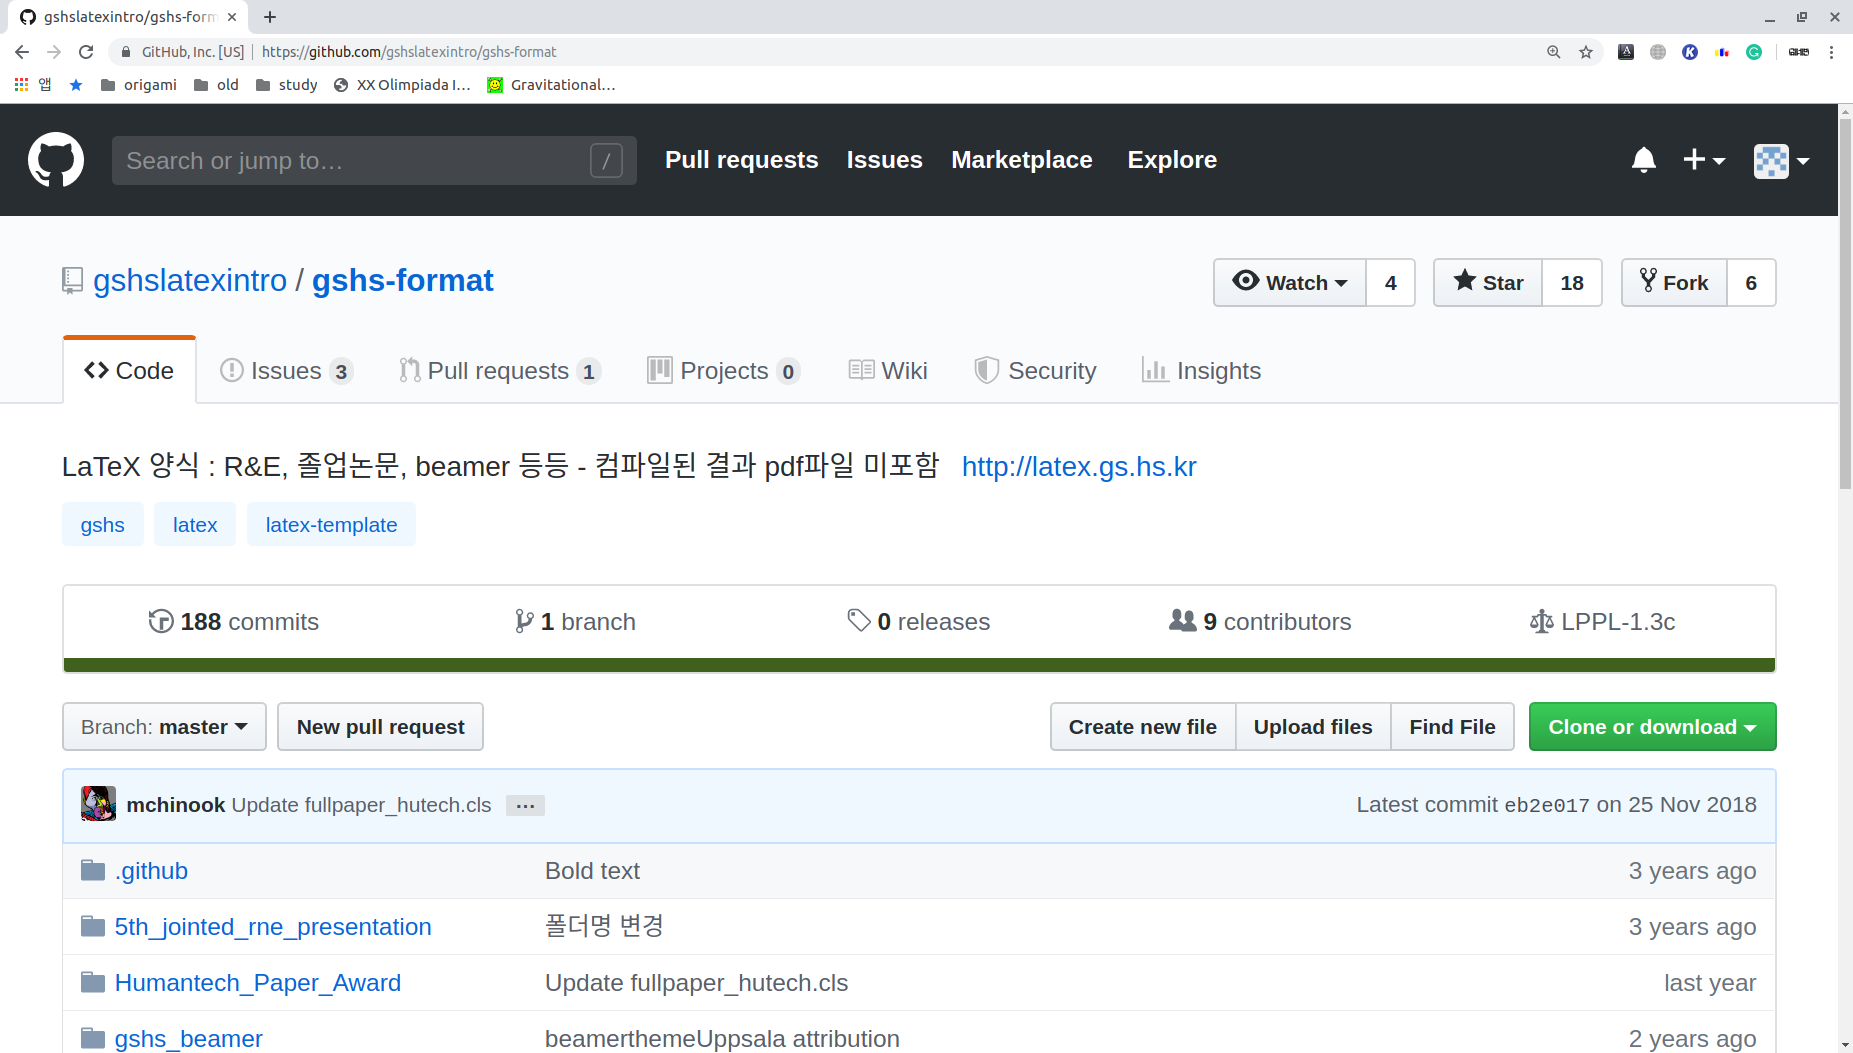
\includegraphics[width=\textwidth]{./pictures/github.png}
	\end{figure}
\end{frame}

\begin{frame}[t]{심화 R\&E, 졸업논문 양식}
	\url{https://github.com/gshslatexintro/gshs-format/tree/master/gshs_rne_report}
	\begin{figure}[h]
		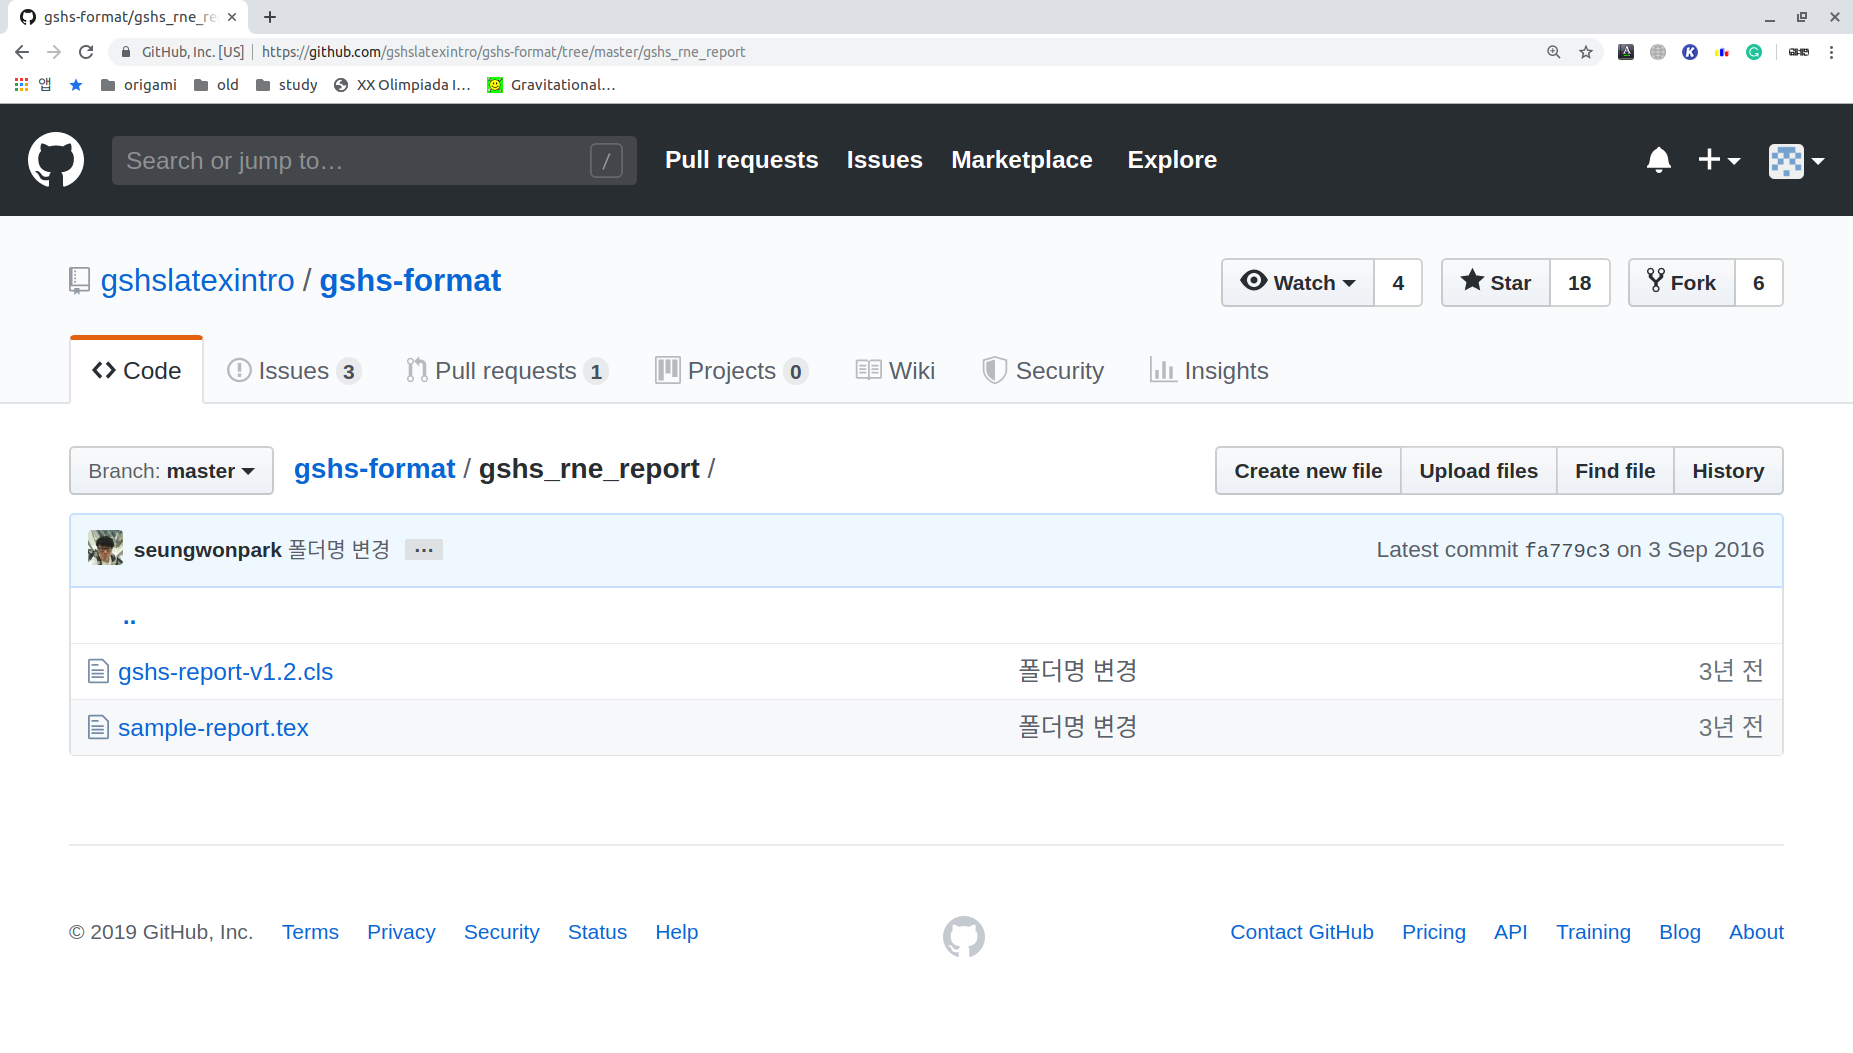
\includegraphics[width=\textwidth]{./pictures/github2.png}
	\end{figure}
\end{frame}

\section{Tips}

\begin{frame}[t]{Tips}
	
	\begin{itemize}
		\item \textbf{Ask Google!} (중요)
		\begin{itemize}
			\item '표의 칸에 대각선 어떻게 넣나요?' : \\
			구글 검색 : 'latex table diagonal line'
			\item 키워드를 모르겠다면, 횡설수설 검색하다가 키워드를 찾고, 그 키워드로 다시 검색하면 된다.
			\item 에러가 발생할 경우, 에러 메시지를 복사해 검색해보자.
		\end{itemize}
		\vskip 1pc
		
		\item 중간중간에 컴파일을 해 본다. \\
		수정 사항이 많은데 에러가 발생할 경우, 찾기가 힘들어짐.
		\vskip 1pc
		\item 긴 단어를 많이 사용해야 할 경우, \texttt{\textbackslash newcommand}를 통해 하나의 명령어로 만들어 버린다.
	\end{itemize}
	
\end{frame}

\begin{frame}[t]{Tips}

\begin{itemize}
	\item \TeX 에 어느 정도 익숙해졌다면...
	\begin{itemize}
		\item \texttt{\textbackslash newcommand}, \texttt{\textbackslash newenvironment}를 통해 새로운 명령어나 환경을 만들어 편하게 작업할 수 있다.
		\item \texttt{.cls} 파일로 클래스를 직접 정의하여 사용할 수 있다.
	\end{itemize}
	\vskip 1pc
	\item 경기과학고 \TeX\ 사용자협회 GitHub에 올라와 있는 다양한 예시들을 참고하자.
\end{itemize}

\end{frame}

\begin{frame}[t]{경기과학고 \TeX\ 사용자협회}
	\begin{figure}[h]
		\centering
		
\includegraphics[width=\textwidth]{./pictures/homepage.png}
	\end{figure}
\end{frame}

\begin{frame}[t]{경기과학고 \TeX\ 사용자협회}
	\setstretch{1.25}
	\begin{itemize}
		\item 2015.7 : 31기 윤지용의 \TeX\ 졸업논문 공개
		\item 2015.8.2: \url{github.com/gshslatexintro} 개설
		\begin{itemize}
			\item 32기 박승원 - 교우 간 \TeX\ 스터디 활동을 위해 개설
		\end{itemize}
		\item 2015.12 :
	\end{itemize}
	\begin{quote}
		"\TeX 사용에 대한 진입 장벽을 없애고, \\
		\TeX 을 사용한다면 누구나 쓸 수 있는 \\
		각종 양식 파일을 공유하고 공동 편집하자!"
	\end{quote}
	\vspace{-.5cm}
	\begin{flushright}
		--- 32기 협회 일동
	\end{flushright}
	$ \rightarrow $ 텍 입문서 제작, 텍 워크샵 진행, 각종 텍 예제 및 양식 제작/배포 등\ldots
\end{frame}

\begin{frame}[t]{경기과학고 \TeX\ 사용자협회}
	\begin{itemize}
		\item 각종 양식 및 입문서, 예시작 온라인 제공
		\begin{itemize}
			\item 주소 : \url{latex.gs.hs.kr}
			\item 지금 보고 있는 이 자료도 홈페이지에서 다운 가능!
		\end{itemize}
		\item 양식
		\begin{itemize}
			\item R\&E, 졸업논문, 휴먼테크, beamer 등
		\end{itemize}
		\item 예시(예제)
		\begin{itemize}
			\item 예제 코드를 보면서 \TeX\ 배우기 (굉장히 중요)
		\end{itemize}
		\vspace{1cm}
		\item {\scriptsize \textbf{다운로드 방법} : \url{latex.gs.hs.kr} - 다운로드 - `다운로드 페이지 링크'}
	\end{itemize}
	
\end{frame}

\begin{frame}[t]{구인 광고}
	\begin{itemize}
		\item 본 협회의 활동에 참여하고 싶다면,
		\begin{itemize}
			\item GitHub에 가입한 뒤
			\item username을 서울 선생님께 발송.
			\item \url{github.com/gshslatexintro} 멤버에 추가
			\item 선생님들께서도 참여 가능합니다.
		\end{itemize}
		\vskip 1pc
		\item 저희선배가 그랬듯이, 저희가 그랬듯이, 양식 제작 등의 활동을 하며 텍을 공부해볼 수 있을 것입니다. 절호의 기회를 놓치지 마세요!
		\begin{itemize}
			\item 5代 회장 및 개발진, 웹마스터 모집.
		\end{itemize}
	\end{itemize}
	
\end{frame}

\end{document}